\chapter{Metodologia}
\label{sec:Metodologia}
Neste capítulo serão descritos os procedimentos utilizados para verificar os efeitos de envelhecimento acelerado nos FPGAs de interesse. Ele será composto por três seções.

A primeira irá apresentar os FPGAs escolhidos para serem estudados, além dos motivos para essa escolha e de características desses dispositivos.

A segunda irá descrever como os osciladores em anel foram projetados, programados e sintetizados nos FPGAs, além de detalhar sobre as decisões tomadas com relação a topologia e número de inversores dos osciladores.

Por fim, a terceira irá detalhar os ensaios realizados utilizando a câmara térmica para estressar os dispositivos e envelhecê-los, bem como as análises e comparações realizadas para alcançar os resultados.

\section{Dispositivos Ensaiados}

Foram utilizadas as placas de desenvolvimento DE2 e ZedBoard. Elas foram escolhidas considerando suas disponibilidades no laboratório e por serem de fabricantes diferentes e possuírem nós tecnológicos diferentes.

A DE2 possui o FPGA XXXXX da família o Cyclone II da fabricante Altera, pertencente a Intel, que possui um nó tecnológico de 90nm. A Zedboard possui o FPGA YYYYYY, da Xilinx, agora pertencente a AMD, que possui um nó tecnológico de 28nm.

Ambas as placas possuem, além dos FPGAs, componentes e periféricos necessários para testes e prototipação de sistemas, como: botões, chaves, LEDs, display, memória flash e ediversas entradas e saídas.
\section{Desenvolvimento dos Osciladores em Anel}

A topologia de oscilador em anel foi escolhida para os testes por sua disseminada utilização na caracterização de dispositivos MOSFET. Seu uso é amplo, pois medidas a utilizando se aproximam muito mais de aplicações reais do que medições paramétricas DC padrões.

Foram realizados testes preliminares com diferentes quantidades de inversores para encontrar uma quantidade apropriada, pois, com poucos osciladores não há tempo suficiente para os inversores chavearem e com muitos osciladores o limite de iterações que as IDEs permitem era atingido.

Considerando isso, foi decidido que em cada um dos dispositivos foi sintetizado dois osciladores, um com 1001 inversores e outro com 4999. A escolha de utilizar dois osciladores em cada FPGA foi tomada por dois motivos: para se ter certeza que as IDEs não estavam simplificando os estágios inversores do circuito sintetizado e para verificar que o envelhecimento afeta igualmente diferentes partes do FPGA.

A grande quantidade de inversores é relevante, pois assim as pequenas variações aleatórias nas características de cada transistor que compõe os dispositivos tenderão a se diluir.

\subsection{Desenvolvimento do Código para os Osciladores}

Para desenvolver e sintetizar os osciladores em anel foi utilizada a linguagem de descrição Verilog. Para o Cyclone II foi utilizada a IDE Quartus II versão 12.1, já para o ZedBoard foi utilizada a IDE Vivado versão 2023.1.

O Quadro \ref{code:RingOsc} mostra o código desenvolvido em Verilog para o módulo que implementa o oscilador em anel com N inversores. O mesmo código foi utilizado para os dois FPGAs nas duas IDEs diferentes.

\begin{lstlisting}[label={code:RingOsc}, style=VerilogStyle, caption={Módulo do Oscilador em Anel. Fonte: O Autor}]
module RingOscillator 
	#(parameter N = 5)
	(
		input  en,
		output reg and_1    /*synthesis keep*/
	);
	reg [N - 1:0] notGate /*synthesis keep*/;
	integer i;
	generate
	  always @ (*) begin
		  and_1 <= en & notGate[N - 1];
	  	notGate[0] <= ~and_1;
	  	for (i = 1; i < N; i = i + 1)   begin: inverter_chain
			  notGate[i] <= ~notGate[i - 1];
		  end
	  end
	endgenerate
endmodule
\end{lstlisting}

O módulo possui uma entrada en, responsável por habilitar o circuito, uma saída and\_1 que é a saída da porta and do circuito, de onde o sinal do oscilador é obtido. O valor N é parametrizável, o que permite a reutilização do mesmo código para osciladores com diferentes números de inversores.

São então instanciadas N registradores, que serão utilizados para criar os inversores. O registrador and\_1 recebe o resultado da operação E lógica do sinal de enable e a saída do último inversor. O primeiro inversor é definido como o registrador and\_1 invertido.

Um bloco 'for' é utilizado para automatizar as atribuições dos inversores seguintes, sendo a cada um atribuído o valor inversor anterior negado.

Um ponto importante de destacar é a necessidade de utilizar diretivas de compilação para impedir que os inversores sejam simplificados na síntese. Essas diretivas são diferentes em cada uma das IDEs, na Quartus II é utilizado a diretiva /* synthesis keep */ e na Vivado é utilizado a diretiva /* synthesis syn\_keep=1 */.

Na Figura \ref{fig:DE2Imp3Osc} pode ser visto como o Quartus II implementa em hardware o código do Quadro \ref{code:RingOsc} para um N igual a 3. A implementação é feita através de portas lógicas comuns, o que é diferente da implementação feita pelo Vivado, como visto na Figura \ref{fig:ZedImp3Osc}, que utiliza LUTs de uma variável para representar os inversores.

\begin{figure}[H]
    \centering
    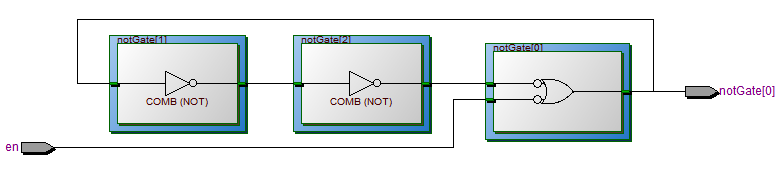
\includegraphics[width=\linewidth]{figures/Metodologia/DE2_Implementation_3Inverter_Gates.png}
    \caption{Síntese do módulo de alto nível gerado no Quatus II. Fonte: O Autor}
    \label{fig:DE2Imp3Osc}
\end{figure}

\begin{figure}[H]
    \centering
    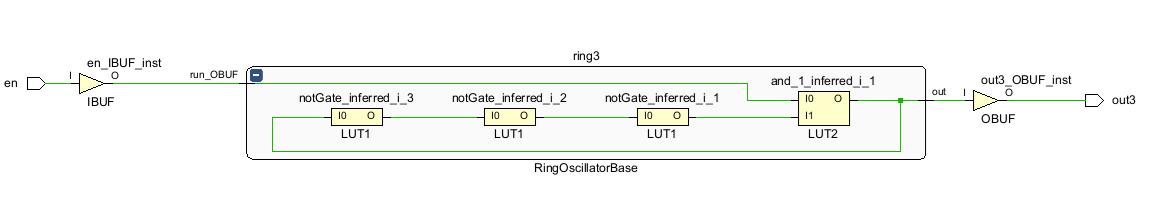
\includegraphics[width=\linewidth]{figures/Metodologia/ZedBoard_Implementation_3Inverter.png}
    \caption{Síntese do módulo de alto nível gerado no Vivado. Fonte: O Autor}
    \label{fig:ZedImp3Osc}
\end{figure}

O Quadro \ref{code:TopLevel} mostra o módulo de alto nível em que é instanciado dois osciladores em anel, um com 1001 e outro de 4999 inversores. 

\begin{lstlisting}[label={code:TopLevel}, style=VerilogStyle, caption={Estanciamento dos Módulos. Fonte: O Autor}]
module TopLevel
	(
		input en,
		output run,
		output out1001, out4999
	);
	
	assign run = en;

	RingOscillator #(.N(1001)) ring1001(en, out1001);
	RingOscillator #(.N(4999)) ring4999(en, out4999);
endmodule
\end{lstlisting}

O módulo possui uma entrada 'en', responsável por habilitar o circuito, uma saída 'run', usada para indicar que o circuito está em funcionamento e as saídas dos dois osciladores 'out1001', 'out4999'. Também são declaradas duas instâncias do módulo desenvolvido no Quadro \ref{code:RingOsc}.

As Figuras \ref{fig:DE2RtlSchem} e \ref{fig:ZedRtlSchem1} mostram, respectivamente, o circuito implementado pelo software Quartus II e Vivado para o módulo de alto nível que serão utilizado nos FPGAs.

\begin{figure}[H]
    \centering
    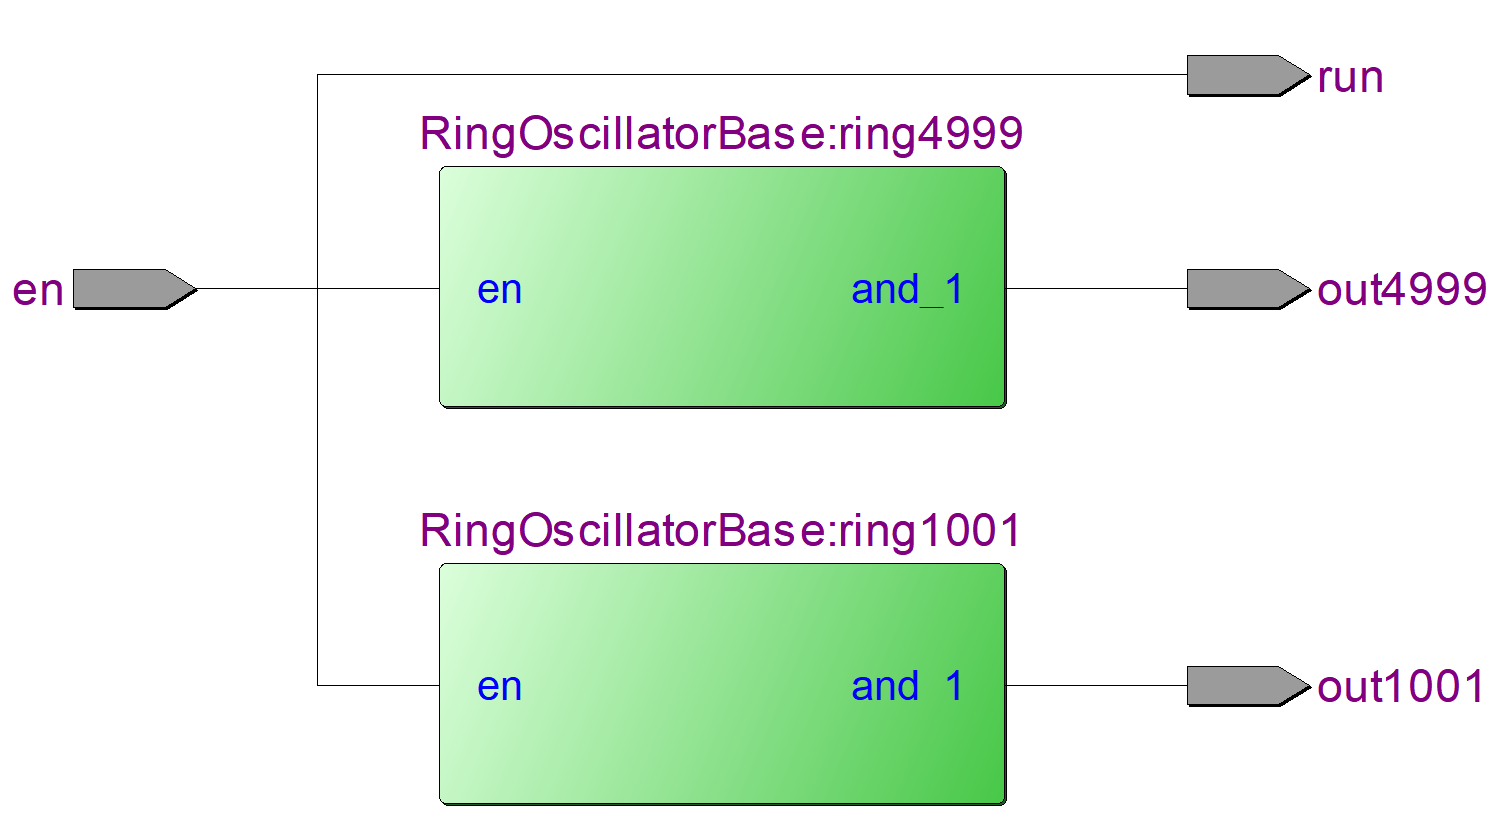
\includegraphics[scale=0.25]{figures/Metodologia/DE2_RTL_Schematic.png}
    \caption{Síntese de um oscilador com três inversores gerado no Quatus II. Fonte: O Autor}
    \label{fig:DE2RtlSchem}
\end{figure}

\begin{figure}[H]
    \centering
    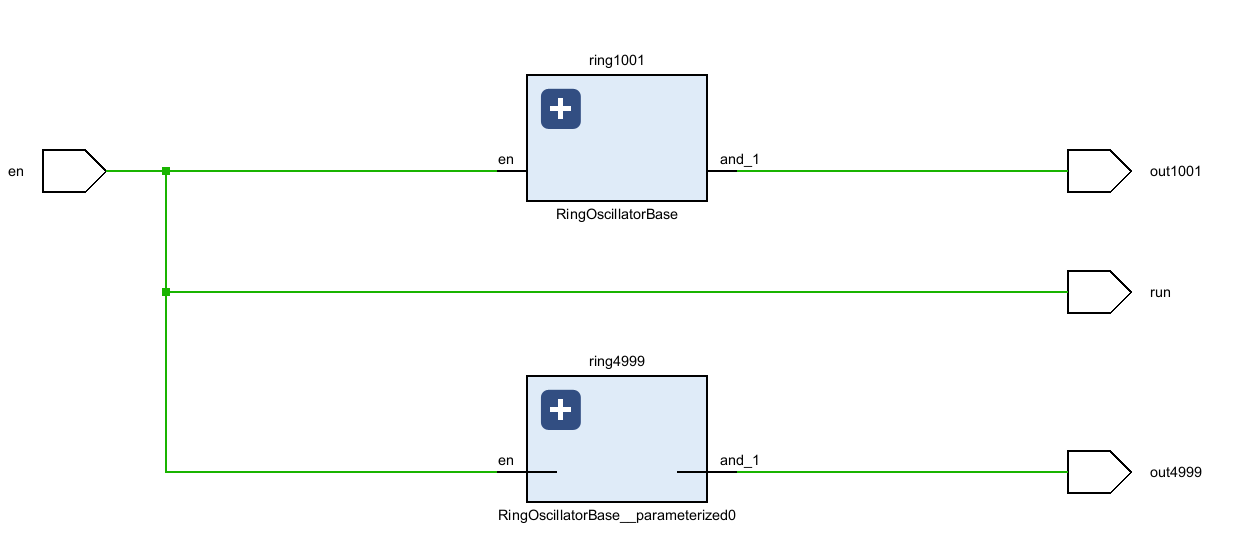
\includegraphics[width=\linewidth]{figures/Metodologia/ZedBoard_RTL_Schematic.png}
    \caption{Síntese de um oscilador com três inversores gerado no Vivado. Fonte: O Autor}
    \label{fig:ZedRtlSchem1}
\end{figure}

Nas duas placas a entrada 'en' foi atribuída a um pino do FPGA ligado a uma chave, a saída 'run' foi atribuída a um pino do FPGA ligado a um LED e as saídas 'out1001' e out4999 foram atribuídas a pinos do FPGA ligados a conectores de entrada e saída de uso geral.

Após o desenvolvimento, o circuito sintetizado foi simulado utilizando a ferramenta apropriada para cada um dos componentes. Constatada a validade da solução ela foi transferida para os FPGAs reais e será medida, através de um osciloscópio, a frequência de oscilação das saídas do circuitos.
\section{Ensaios de Envelhecimento}

Para induzir o fenômeno de BTI nos dispositivos foi utilizada uma câmara térmica para ensaios com componenentes eletrônicos. Inicialmente a temperatura de exposição foi de 100°C, temperatura que é inferior a faixa de ocorrência do BTI, mas que foi utilizada para verificar se os componentes não iriam ser danificados com a temperatura.

A Figura \ref{fig:CamTerm} mostra a câmera térmica utilizada para os ensaios. Ele foi fabricado pela SPX Thermal Product Solutions e alcança temperaturas de -75ºC a 200ºC

\begin{figure}[H]
    \centering
    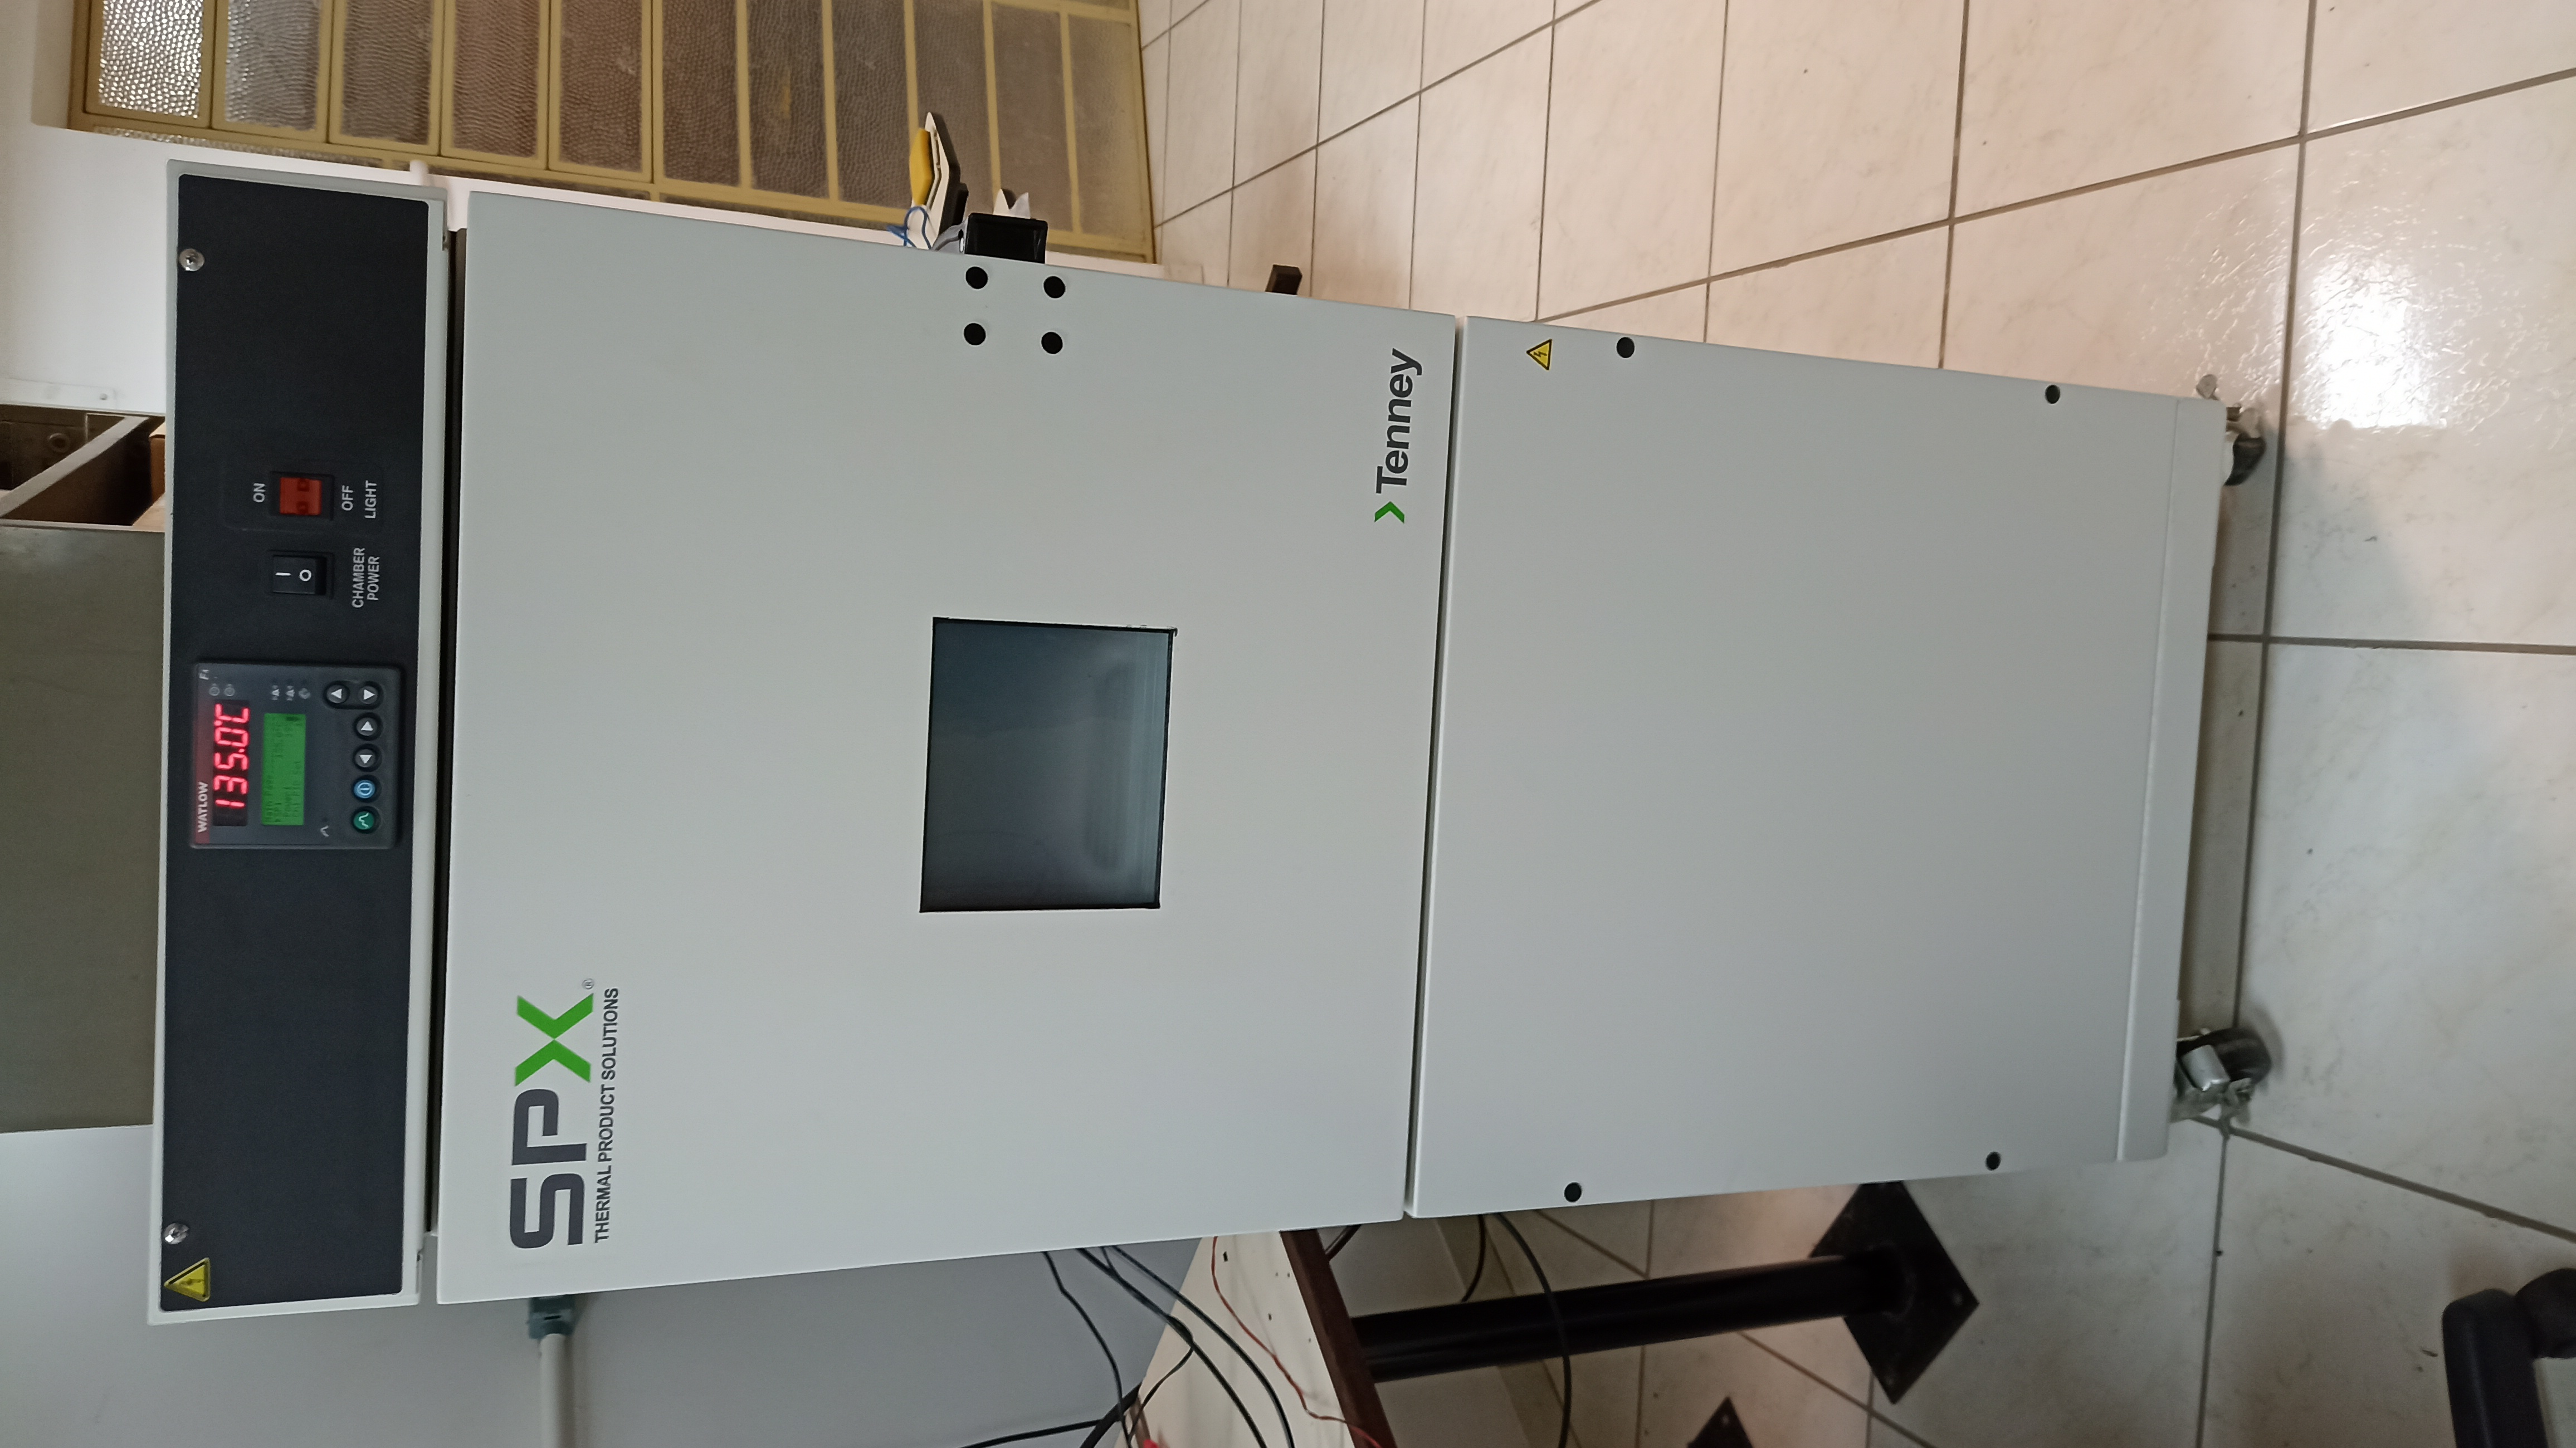
\includegraphics[angle=270, scale=0.08]{figures/Ensaios_CamaraTermica.jpg}
    \caption{Câmara térmica utilizada para os ensaios. Fonte: O Autor}
    \label{fig:CamTerm}
\end{figure}

Constatando que não houve problema à 100ºC, a temperatura foi aumentada para 125°C. Como também não houve danos, a temperatura foi, então, elevada para 135°C.

Nessa temperatura foi observado que o conector de alimentação da placa DE2 apresentava sinais de derretimento, por isso, a temperatura dos ensaios foi definida em 135°C. Temperatura que está dentro da faixa de 125 e 175ºC que a bibliografia indica como sendo a faixa em que o BTI ocorre mais facilmente.

O tempo que os dispositivos forem expostas ao calor não foi contínua, devido a impossibilidade de ficar durante a noite no laboratório e, por motivos de segurança, de deixar a câmara térmica ligada sem supervisão. Portanto os dispositivos, de forma geral, foram expostos à câmara térmica durante o dia e retirados dela durante a noite, ficando ligados o tempo todo, de forma que não houvesse relaxamento.

Outras duas placas, dos mesmo modelos das ensaiadas, foram deixadas fora da câmara térmica pelo mesmo tempo, sempre ligadas e com os mesmos osciladores em anel sintetizados. Comparar as medidas entre as placas que foram aquecidas com as que nao foram é importante para verificar que se a degradação na frequência é proveniente do estresse térmico ou se é apenas resultado do funcionamento prolongado.

A câmara térmica permite realizar medidas nos dispositivos ensaiados enquanto eles estão dentro dela. Portanto foi possível medir a frequência dos osciladores em anel durante o processo de estresse térmico.

Enquanto a câmara aquece da temperatura ambiente pra temperatura alvo, as medições foram mais frequentes, de cinco em cinco minutos. Quando a temperatura alvo é atingida as medidas ficam mais esparsas.

É importante separar os efeitos instantâneos da temperatura na frequência dos osciladores do efeito a longo prazo do BTI. Por isso é necessário comparar as medidas feitas em uma mesma temperatura. O momento que a temperatura é a mais estável é quando a câmara já chegou aos 135°C.

Outra comparação relevante é a das curvas frequência por temperatura ao longo de cada ciclo.

Comparando essas medidas em relação ao tempo total estressado será possível constatar se houve ou não uma degradação na frequência de funcionamento dos dispositivos. E se houve uma diferença significativa na degradação entre as duas placas.

Após os ensaios de envelhecimento foi realizado um ensaio para medir a recuperação dos circuitos, para verificar quanto da degradação sofrida é reversível. Para isso as quatro placas foram desligadas e deixadas em temperatura ambiente. Medidas ao longo do tempo foram realizadas até o tempo de relaxamento totalizar o tempo total que as placas foram estressadas.

\begin{figure}[H]
    \centering
    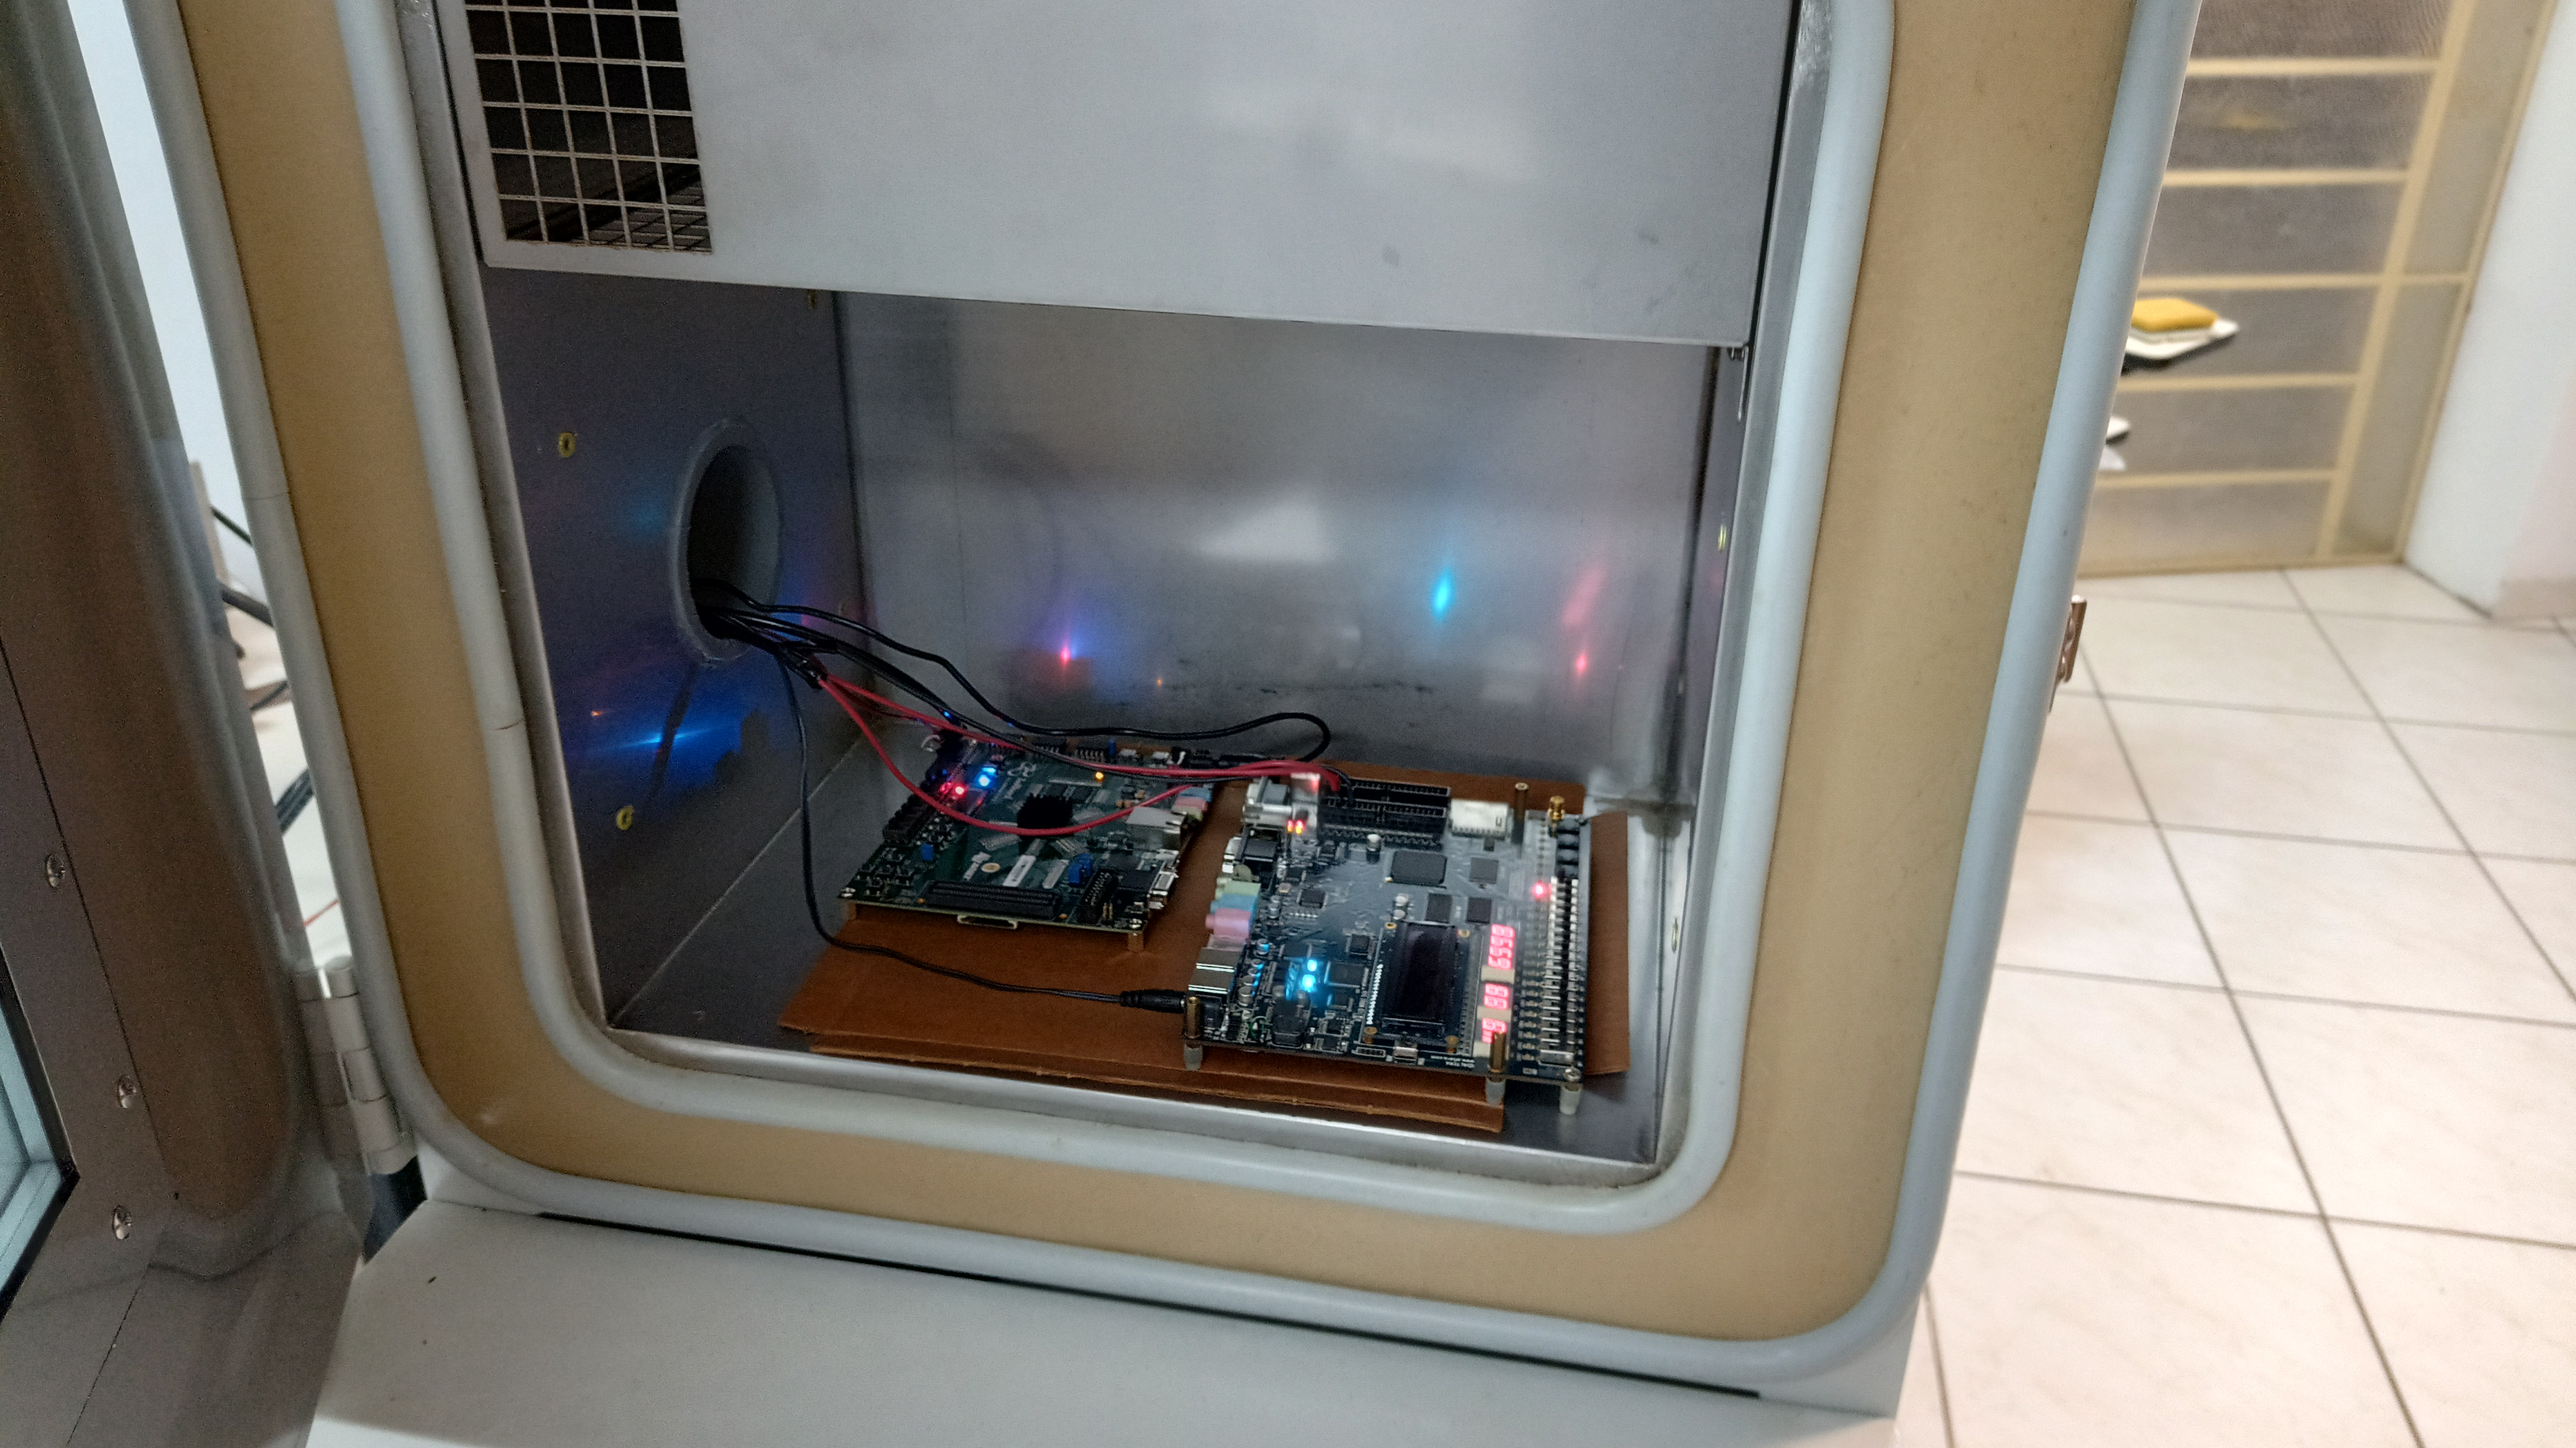
\includegraphics[width=\linewidth]{figures/Ensaios_FpgasNoForno.jpg}
    \caption{FPGAs dentro da Câmara térmica. Fonte: O Autor}
    \label{fig:CamTerm}
\end{figure}

\begin{figure}[H]
    \centering
    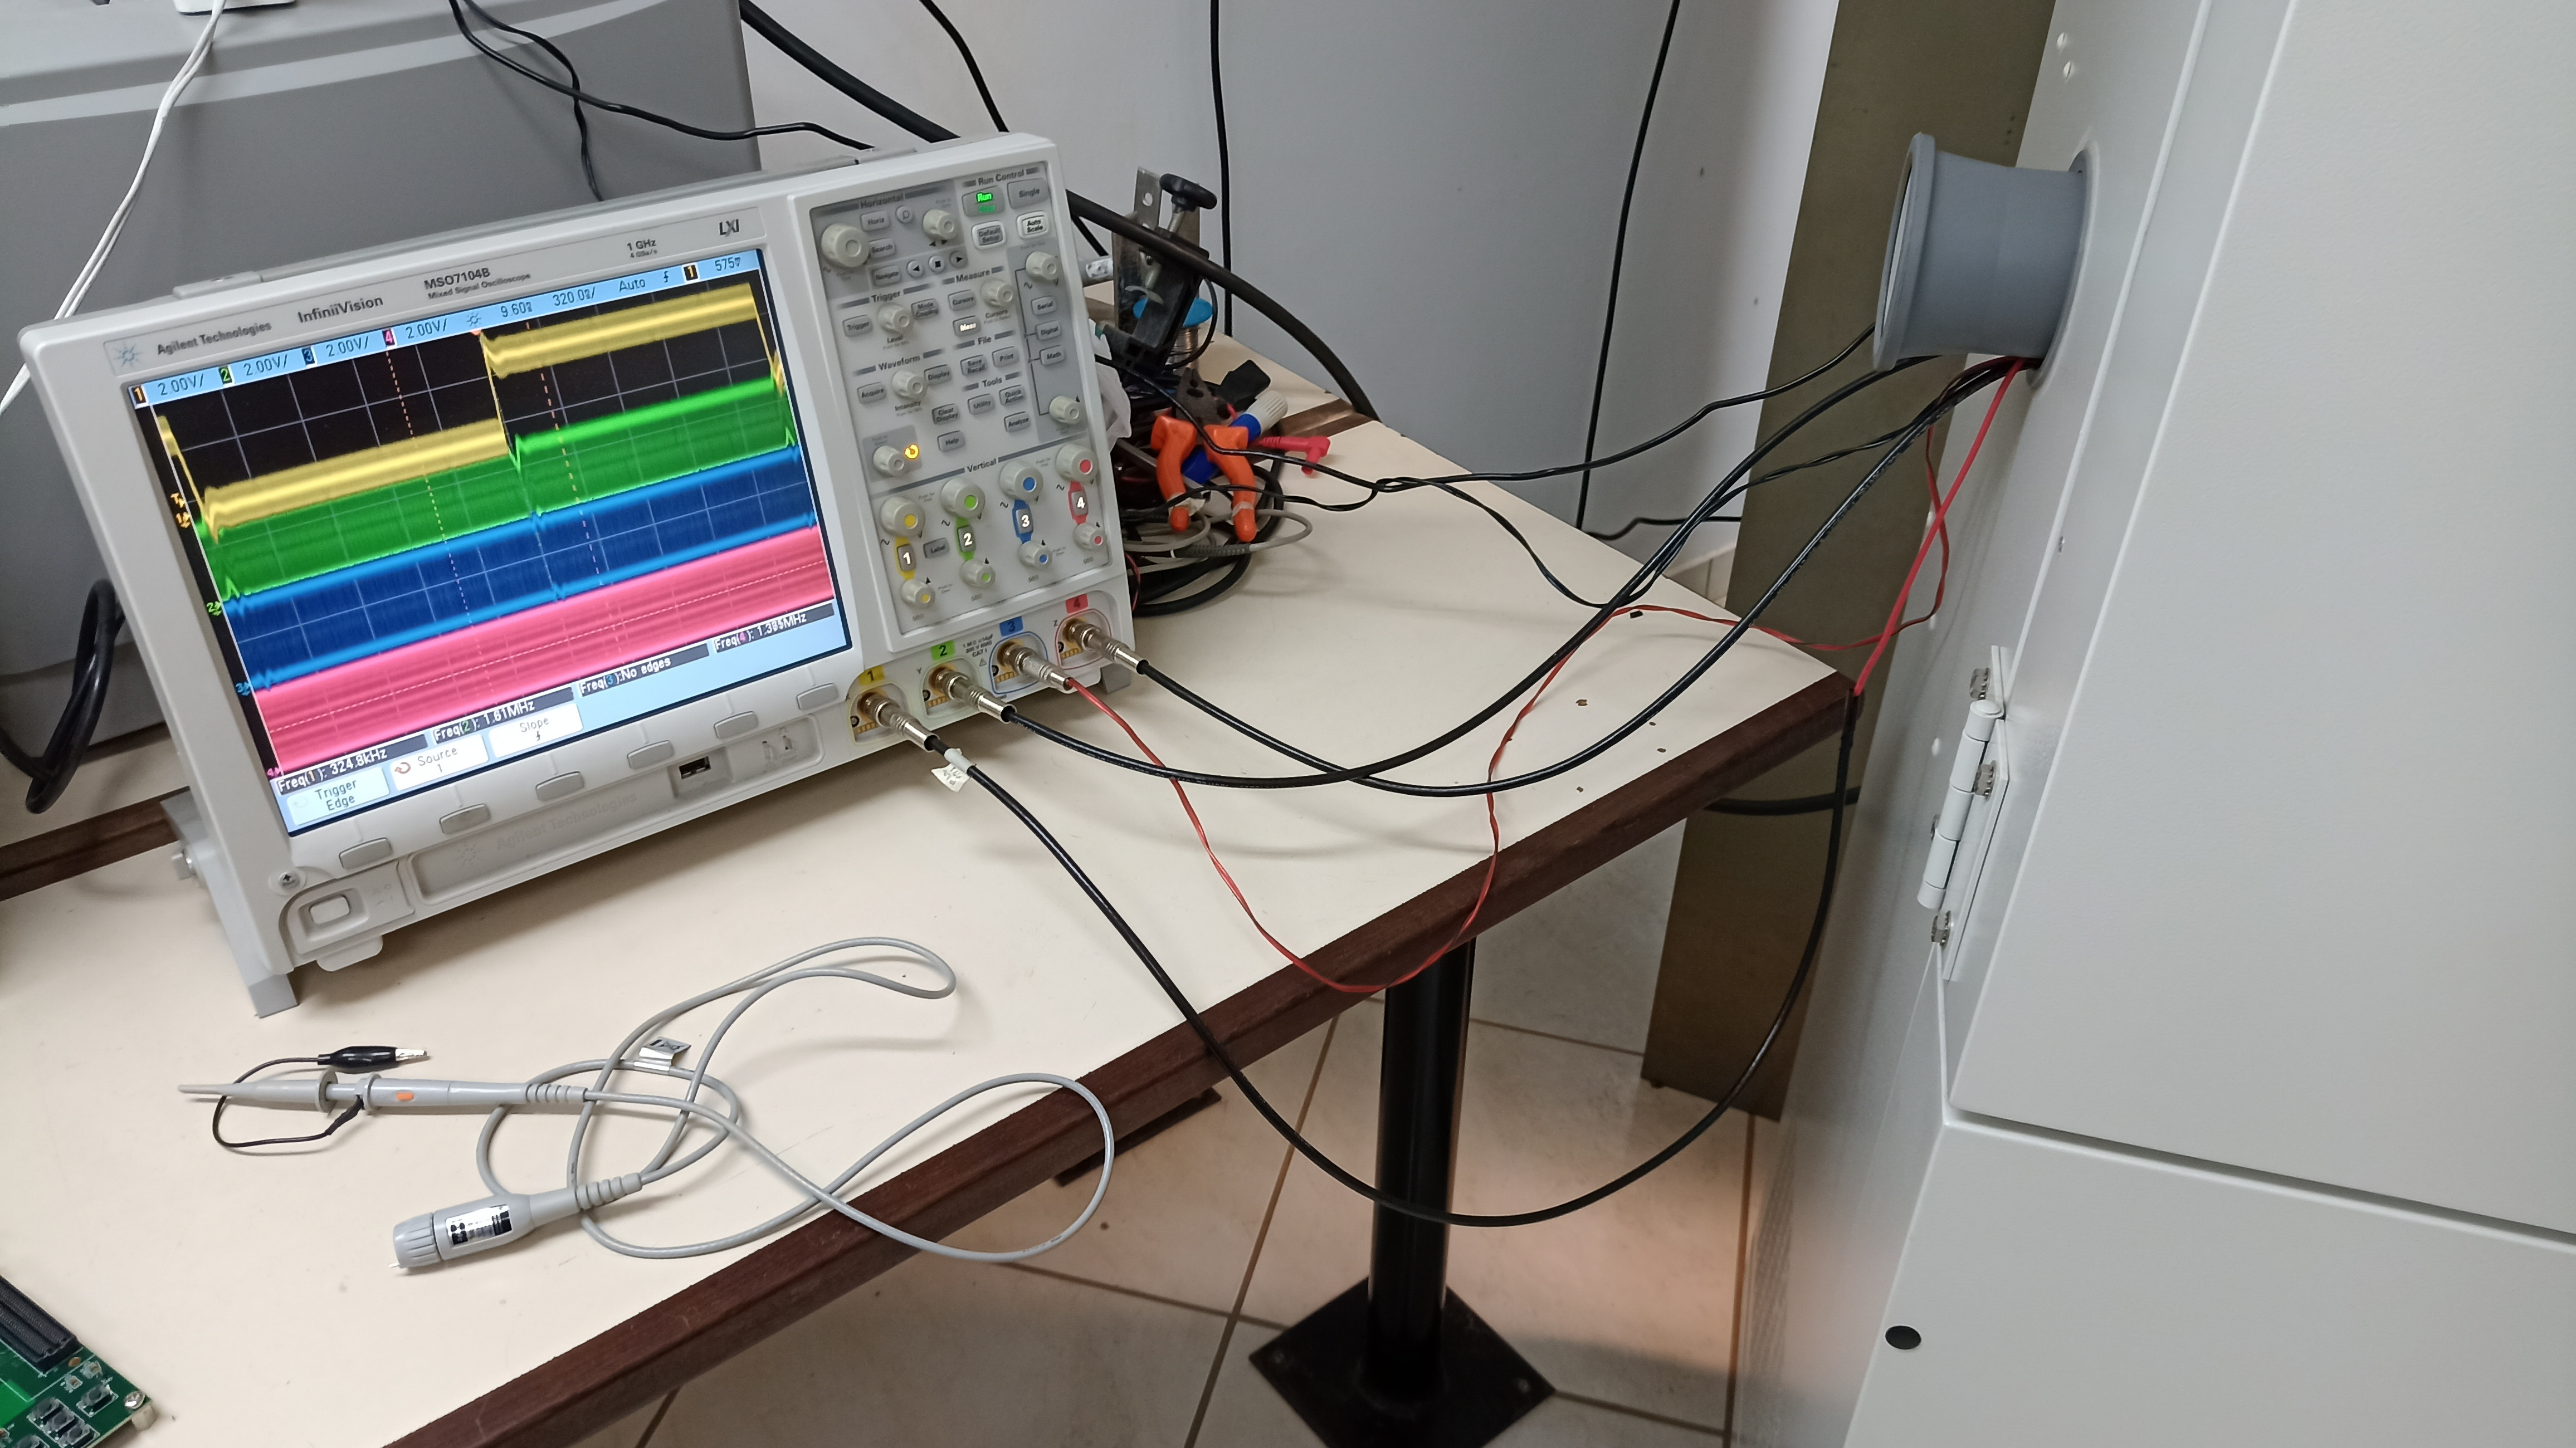
\includegraphics[width=\linewidth]{figures/Ensaios_Osciloscopio.jpg}
    \caption{Osciloscópio utilizado para as medidas. Fonte: O Autor}
    \label{fig:CamTerm}
\end{figure}

